% -*- mode: latex; -*- mustache tags:  
\documentclass[10pt,twoside,english]{_support/latex/sbabook/sbabook}
\let\wholebook=\relax

\usepackage{import}
\subimport{_support/latex/}{common.tex}

%=================================================================
% Debug packages for page layout and overfull lines
% Remove the showtrims document option before printing
\ifshowtrims
  \usepackage{showframe}
  \usepackage[color=magenta,width=5mm]{_support/latex/overcolored}
\fi


% =================================================================
\title{A PharoThings Tutorial}
\author{Allex Oliveira}
\series{Square Bracket tutorials}

\hypersetup{
  pdftitle = {A PharoThings Tutorial},
  pdfauthor = {Allex Oliveira},
  pdfkeywords = {IoT, Raspberry, PharoThings, Pharo}
}


% =================================================================
\begin{document}

% Title page and colophon on verso
\maketitle
\pagestyle{titlingpage}
\thispagestyle{titlingpage} % \pagestyle does not work on the first one…

\cleartoverso
{\small

  Copyright 2017 by Allex Oliveira.

  The contents of this book are protected under the Creative Commons
  Attribution-ShareAlike 3.0 Unported license.

  You are \textbf{free}:
  \begin{itemize}
  \item to \textbf{Share}: to copy, distribute and transmit the work,
  \item to \textbf{Remix}: to adapt the work,
  \end{itemize}

  Under the following conditions:
  \begin{description}
  \item[Attribution.] You must attribute the work in the manner specified by the
    author or licensor (but not in any way that suggests that they endorse you
    or your use of the work).
  \item[Share Alike.] If you alter, transform, or build upon this work, you may
    distribute the resulting work only under the same, similar or a compatible
    license.
  \end{description}

  For any reuse or distribution, you must make clear to others the
  license terms of this work. The best way to do this is with a link to
  this web page: \\
  \url{http://creativecommons.org/licenses/by-sa/3.0/}

  Any of the above conditions can be waived if you get permission from
  the copyright holder. Nothing in this license impairs or restricts the
  author's moral rights.

  \begin{center}
    
\includegraphics[width=0.2\textwidth]{_support/latex/sbabook/CreativeCommons-BY-SA.pdf}
  \end{center}

  Your fair dealing and other rights are in no way affected by the
  above. This is a human-readable summary of the Legal Code (the full
  license): \\
  \url{http://creativecommons.org/licenses/by-sa/3.0/legalcode}

  \vfill

  % Publication info would go here (publisher, ISBN, cover design…)
  Layout and typography based on the \textcode{sbabook} \LaTeX{} class by Damien
  Pollet.
}


\frontmatter
\pagestyle{plain}

\tableofcontents*
\clearpage\listoffigures

\mainmatter

\chapter{Lesson 3 - LED Flowing Lights}
Now we can play with the LEDs, turn them on, off, and blink. Let's put 8 LEDs on the breadboard and create a code to turn on/off one at a time. As we did in the last lesson, let's write the first code in playground and then create a class with methods to better control the flow of LED lights.
\section{What we need?}
We are using the lesson 1 setup, but let's use 8 LEDs and 8 resistors.
\subsection{Components}
\begin{itemize}
\item 1 Raspberry Pi connected to your network (wired or wireless)
\item 1 Breadboard
\item 8 LEDs
\item 8 Resistors 330ohms
\item Jumper wires
\end{itemize}
\section{Experimental procedure}
We saw in the lesson 1 how to connect the LED and resistors on the breadboard. Now let's do the same, but putting more 7 LEDs and resistors on the breadboard.

\begin{itemize}
\item Connect the Ground PIN from Raspberry in the breadboard blue rail (-). 
\item Then connect the 8 resistors from the blue rail (-) to a column on the breadboard, as shown below;
\item Now push the LED legs into the breadboard, with the long leg (with the kink) on the right;
\item And insert the jumper wires connecting the rigth column of each LED to GPIO from 0 to 7, as shown in the Picture \ref{Physical8Leds}.
\end{itemize}

The Figure \ref{Physical8Leds} shows how the electric connection is made:


\begin{figure}

\begin{center}
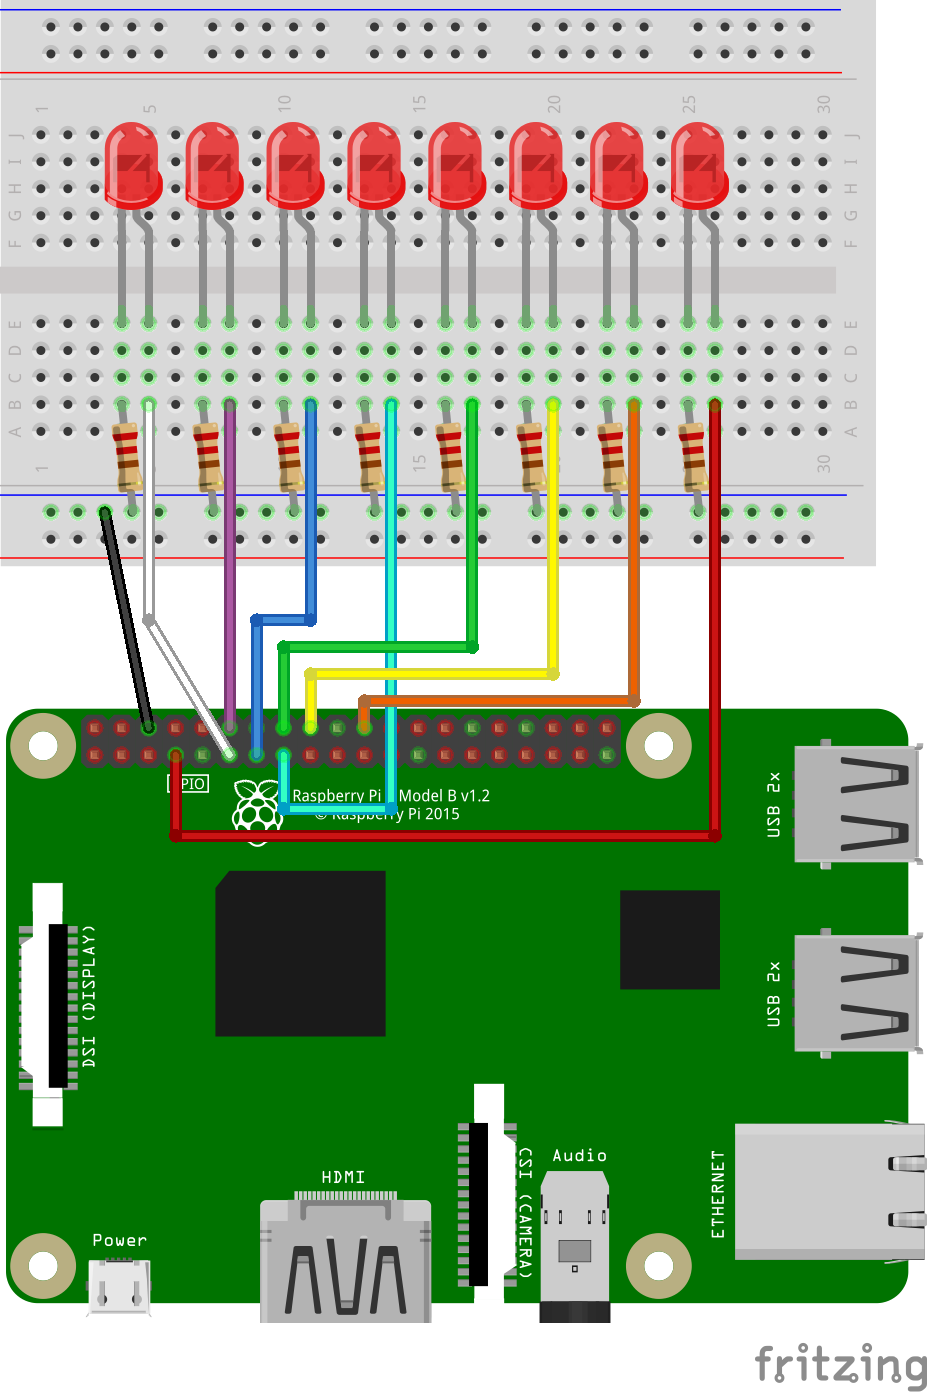
\includegraphics[width=0.6\textwidth]{/Users/allexoliveira/PharoThingsBook/Booklet-APharoThingTutorial/_result/pdf/Chapters/Chap5LEDFlowingLights/figures/pharothings-raspberry-8leds-8resistors-lesson-01.png}\caption{Physical connection 8 LEDs.\label{Physical8Leds}}\end{center}
\end{figure}

\subsection{Connecting remotely}
Through your local Pharo image, let's connect in the Pharo image by running on Raspberry, enable the auto-refresh feature of the inspector, and open the inspector.

Run this code in your local playground:

\begin{displaycode}{plain}
remotePharo := TlpRemoteIDE connectTo: (TCPAddress ip: #[193 51 236 212] port: 40423)
GTInspector enableStepRefresh.
remoteBoard := remotePharo evaluate: [ RpiBoardBRev1 current].
remoteBoard inspect.
\end{displaycode}
\section{Experimental code}
In your inspect window (Inspector on a PotRemoteBoard), let's initialize the 8 LEDs and set the GPIOs to be in digital output mode:

\begin{displaycode}{plain}
code...
\end{displaycode}

To blink the LED let's create a simple loop to change the value of the LED every 1 second by 10 times. To change the value of the object (led value), let's call the method \textcode{toggleDigitalValue}, as we saw previously:

\begin{displaycode}{plain}
code...
\end{displaycode}


% lulu requires an empty page at the end. That's why I'm using
% \backmatter here.
\backmatter

% Index would go here

\end{document}
